\documentclass[]{article}
\usepackage{lmodern}
\usepackage{amssymb,amsmath}
\usepackage{ifxetex,ifluatex}
\usepackage{fixltx2e} % provides \textsubscript
\ifnum 0\ifxetex 1\fi\ifluatex 1\fi=0 % if pdftex
  \usepackage[T1]{fontenc}
  \usepackage[utf8]{inputenc}
\else % if luatex or xelatex
  \ifxetex
    \usepackage{mathspec}
  \else
    \usepackage{fontspec}
  \fi
  \defaultfontfeatures{Ligatures=TeX,Scale=MatchLowercase}
\fi
% use upquote if available, for straight quotes in verbatim environments
\IfFileExists{upquote.sty}{\usepackage{upquote}}{}
% use microtype if available
\IfFileExists{microtype.sty}{%
\usepackage{microtype}
\UseMicrotypeSet[protrusion]{basicmath} % disable protrusion for tt fonts
}{}
\usepackage[margin=1in]{geometry}
\usepackage{hyperref}
\hypersetup{unicode=true,
            pdftitle={Estimating ABO-Gene Allele Frequencies in Population using Phenotypic Blood-Type Data.},
            pdfauthor={Student: Faizan Khalid Mohsin; Professor Lei Sun; Course: CHL5224 Statistical Genetics},
            pdfborder={0 0 0},
            breaklinks=true}
\urlstyle{same}  % don't use monospace font for urls
\usepackage{longtable,booktabs}
\usepackage{graphicx,grffile}
\makeatletter
\def\maxwidth{\ifdim\Gin@nat@width>\linewidth\linewidth\else\Gin@nat@width\fi}
\def\maxheight{\ifdim\Gin@nat@height>\textheight\textheight\else\Gin@nat@height\fi}
\makeatother
% Scale images if necessary, so that they will not overflow the page
% margins by default, and it is still possible to overwrite the defaults
% using explicit options in \includegraphics[width, height, ...]{}
\setkeys{Gin}{width=\maxwidth,height=\maxheight,keepaspectratio}
\IfFileExists{parskip.sty}{%
\usepackage{parskip}
}{% else
\setlength{\parindent}{0pt}
\setlength{\parskip}{6pt plus 2pt minus 1pt}
}
\setlength{\emergencystretch}{3em}  % prevent overfull lines
\providecommand{\tightlist}{%
  \setlength{\itemsep}{0pt}\setlength{\parskip}{0pt}}
\setcounter{secnumdepth}{0}
% Redefines (sub)paragraphs to behave more like sections
\ifx\paragraph\undefined\else
\let\oldparagraph\paragraph
\renewcommand{\paragraph}[1]{\oldparagraph{#1}\mbox{}}
\fi
\ifx\subparagraph\undefined\else
\let\oldsubparagraph\subparagraph
\renewcommand{\subparagraph}[1]{\oldsubparagraph{#1}\mbox{}}
\fi

%%% Use protect on footnotes to avoid problems with footnotes in titles
\let\rmarkdownfootnote\footnote%
\def\footnote{\protect\rmarkdownfootnote}

%%% Change title format to be more compact
\usepackage{titling}

% Create subtitle command for use in maketitle
\providecommand{\subtitle}[1]{
  \posttitle{
    \begin{center}\large#1\end{center}
    }
}

\setlength{\droptitle}{-2em}

  \title{Estimating ABO-Gene Allele Frequencies in Population using Phenotypic
Blood-Type Data.}
    \pretitle{\vspace{\droptitle}\centering\huge}
  \posttitle{\par}
    \author{Student: Faizan Khalid Mohsin; Professor Lei Sun; Course: CHL5224
Statistical Genetics}
    \preauthor{\centering\large\emph}
  \postauthor{\par}
      \predate{\centering\large\emph}
  \postdate{\par}
    \date{September 22, 2020}

\usepackage{booktabs}
\usepackage{longtable}
\usepackage{array}
\usepackage{multirow}
\usepackage{wrapfig}
\usepackage{float}
\usepackage{colortbl}
\usepackage{pdflscape}
\usepackage{tabu}
\usepackage{threeparttable}
\usepackage{threeparttablex}
\usepackage[normalem]{ulem}
\usepackage{makecell}

\begin{document}
\maketitle

\section{Introduction}\label{introduction}

The ABO-gene (ABO locus) on chromosome 9 can have 3 alleles (antigens:
A, B, O). Different pairings of these alleles (AA, AB, BB, AO, etc.)
lead to four phenotypic manifestations in the form of 4 blood types: A,
B, AB, O.

We want to estimate the frequency of the 3 alleles A, B, O in the
population. One way to do this would be to take blood samples of a big
sample from the population of interest and using DNA sequencing to
determine the allele type (A or B or O). However, to get reliable
frequency estimates one needs to do DNA sequencing of a large number of
people, which will be extremely expensive and time consuming. A more
practical and more efficient method for estimating the 3 allele
frequencies of a population would be to collect the phenotypic data (the
blood type A, B, AB or O) and use some statistical method to estimate
the 3 allele frequencies.

In this paper we will layout two separate algorithms and approaches for
the estimations the allele frequency using phenotypic blood type data.
Finally, we will use the actual blood type data gathered from a large
sample of 21104 people from Berlin to demonstrate and estimate the
allele frequency using the two algorithms.

\section{Methods}\label{methods}

We use two methods for approximating the population allele frequencies:
Expectation-Maximization method and Newton-Raphson method.

In the ideal case we could sample n people and find out how many people
possess allele A (\(n_A\)), B (\(n_B\)) and O (\(n_O\)). In such a case
it would be very easy to calculate the allele frequency in the
population:
\(freq(A) = n_A/n, \: \: freq(B) = n_B/n,\: \: and \: \:freq(O) = n_O/n\).
However, getting \(n_A, n_B, n_O\) directly from DNA sequencing is very
expensive and time consuming. It is much easier to collect the blood
type of each individual. This will give us a numeric count of how many
people have each blood type:

\begin{itemize}
\tightlist
\item
  \(n_A\): number of people with blood type A,
\item
  \(n_B\): number of people with blood type B,
\item
  \(n_{AB}\): number of people with blood type AB,
\item
  \(n_O\): number of people with blood type O.
\end{itemize}

We use genetics to link the number of individuals with alleles
\(n_A, n_B, \: and\: \: n_O\) with number of people with phenotypes
\(n_A, n_B, n_{AB}, \:and\: \: n_O\) (blood-type).

\subsection{Genetical Theory and
Notation:}\label{genetical-theory-and-notation}

For estimating the frequency of the three alleles let:

\[p=freq(\mbox{allele } A),\] \[q=freq(\mbox{allele } B),\]
\[o=freq(\mbox{allele } O)= 1-p-q .\]

Now using Hardy--Weinberg equilibrium assumption we get the following
equations:

\[freq(AA)=p^2, \: \:  freq(AO)=2p(1-p-q), \: \:  freq(BB)=q^2, \: \: freq(BO)=2q(1-p-q), \: \:  freq(AB)=2pq, \: \: freq(OO)=(1-p-q)^2.\]

From genetic theory we know that alleles A, B are dominant to allele O;
alleles A, B are co-dominant; and allele O is recessive to alleles A, B.
Using this we get the below mapping from genotype to phenotype:

\begin{longtable}[]{@{}cc@{}}
\toprule
Genotype & Phenotype\tabularnewline
\midrule
\endhead
AA or AO & A\tabularnewline
BB or BO & B\tabularnewline
AB & AB\tabularnewline
OO & 0\tabularnewline
\bottomrule
\end{longtable}

Using the mapping above from allele types (A, B, O), to phenotypic blood
type data (A, B, AB, O) we have the following relationships:

\begin{itemize}
\tightlist
\item
  Blood-Type A: \(n_A=n_{AA}+n_{AO}\),
\item
  Blood-Type B: \(n_B=n_{BB}+n_{BO}\),
\item
  Blood-Type AB: \(n_{AB}=n_{AB}\)
\item
  Blood-Type O: \(n_{O}=n_{OO}\).
\end{itemize}

With the HWE equations and the above mapping from genotypic data to
phenotypic data we get the following formulas for the 4 phenotypic
Blood-Type frequencies:

\[freq(A)=p^2+2p(1-p-q),  \: \:   freq(B)=q^2+2q(1-p-q),\]

\[freq(AB)=2pq,  \: \:   freq(O)=(1-p-q)^2.\]

Although, not all populations satisfy the HWE completely, it is still a
good approximation and a reasonable assumption to make in most cases.

\subsection{Statistical Theory and Likelihood
function:}\label{statistical-theory-and-likelihood-function}

From the notes of Professor Lei Sun\textsuperscript{1}, using the above
theory and notation with the assumption of Hardy-Weinberg Equilibrium
the log likelihood function is:

\[ln(L) \sim n_\text{A}\ln\left(p^2+2\left(-p q+1\right)p\right)+n_\text{AB}\ln\left(2qp\right)+2n_\text{O}\ln\left(-p-q+1\right)+n_\text{B}\ln\left(2q\left(-p-q+1\right)+q^2\right)
\]

Good estimates of p and q can be found by finding the values that
maximize the log-likelihood function. This can be done by taking the
full first derivative, equating it to zero and then solving for p and q.
However, this is very difficult to do analytically. Hence, we will use
two different algorithms and approaches to estimate p and q. Namely, the
Newton-Raphson algorithm and the Estimation-Maximization algorithm.

\subsubsection{Newton-Raphson Algorithm
Method}\label{newton-raphson-algorithm-method}

We directly find the maximum of the log-likelihood function using
Newton-Raphson algorithm. It is a numerically computational iterative
method to find a function's maxima.

Let: \[f(\vec \theta) = lnL(p,q) = f(p,q)\]

To approximate the values of \(\hat{p}, \hat{q}.\) We need to get the
full first derivatives with respect to p and q.

Hence, first take the first derivatives (gradient vector):

\[ f'(\vec \theta) = f'(p,q) = 
\left[ \begin{array}{c} 
\frac{\partial{f(p,q)}}{\partial{p}}\\
\frac{\partial{f(p,q)}}{\partial{q}}
\end{array} \right] \]

However, before we take the first derivatives, we can simplify our
log-likelihood function, making it very easy to take the derivatives in
practice.

Using the properties of log and simple arithmetic we get the following
simplified version of the log-likelihood function:

\[ln(L) \sim n_\text{B}\ln\left(2p+q-2\right)+n_\text{A}\ln\left(p+2q-2\right)+n_\text{AB}\ln\left(p\right)+n_\text{A}\ln\left(-p\right)+2n_\text{O}\ln\left(-p-q+1\right)+n_\text{AB}\ln\left(2q\right)+n_\text{B}\ln\left(-q\right)
\]

Now using the chain rule \((f(g(x)))' = f'(g(x))g'(x)\) and the fact
that the derivative of \(ln(x)\) is \(1/x\), it is very easy to get the
partial derivatives with respect to p and q.

where:

\[ \frac{\partial f}{\partial p } = \dfrac{2n_\text{B}}{2p+q-2}+n_\text{A}\left(\dfrac{1}{p+2q-2}+\dfrac{1}{p}\right)+\dfrac{n_\text{AB}}{p}-\dfrac{2n_\text{O}}{-p-q+1}
\]

\[\frac{\partial f}{\partial q } = \dfrac{2n_\text{A}}{2q+p-2}+n_\text{B}\left(\dfrac{1}{q+2p-2}+\dfrac{1}{q}\right)+\dfrac{n_\text{AB}}{q}-\dfrac{2n_\text{O}}{-q-p+1}
\]

Now we also need to take the second derivatives (Hessian matrix):

\[ f''(\vec \theta) = f''(p,q) = 
\left[ \begin{array}{cc} 
\frac{\partial^2 {f(p,q)}}{{\partial{p}}^2}&
\frac{\partial^2 {f(p,q)}}{\partial{p}\partial{q}}\\
\frac{\partial^2 {f(p,q)}}{\partial{q}\partial{p}}&
\frac{\partial^2 {f(p,q)}}{{\partial{q}}^2}
\end{array} \right] \]

Using again the chain rule and the reciprocal rule that:
\((1/f(x))' = -f'(x)/f(x)^2\) the following second partial derivatives
are easily found:

\[ \frac{\partial^2 f}{\partial p^2} = -\dfrac{4n_\text{B}}{\left(2p+q-2\right)^2}+n_\text{A}\left(-\dfrac{1}{\left(p+2q-2\right)^2}-\dfrac{1}{p^2}\right)-\dfrac{n_\text{AB}}{p^2}-\dfrac{2n_\text{O}}{\left(-p-q+1\right)^2}
\]

\[ \frac{\partial^2 f}{\partial q^2} = -\dfrac{4n_\text{A}}{\left(2q+p-2\right)^2}+n_\text{B}\left(-\dfrac{1}{\left(q+2p-2\right)^2}-\dfrac{1}{q^2}\right)-\dfrac{n_\text{AB}}{q^2}-\dfrac{2n_\text{O}}{\left(-q-p+1\right)^2}
\]

\[\frac{\partial^2 f}{\partial q \partial p } = -\dfrac{2n_\text{B}}{\left(2p+q-2\right)^2}-\dfrac{2n_\text{A}}{\left(p+2q-2\right)^2}-\dfrac{2n_\text{O}}{\left(-p-q+1\right)^2}
\]

\[\frac{\partial^2 f}{\partial p \partial q } =-\dfrac{2n_\text{B}}{\left(2p+q-2\right)^2}-\dfrac{2n_\text{A}}{\left(p+2q-2\right)^2}-\dfrac{2n_\text{O}}{\left(-p-q+1\right)^2}
\]

Now choose a starting value:
\[\vec \theta ^{(0)} = (p^{(0)}, q^{(0)})\].

For \(k=1,2,...\) the updating function is:

\[\vec \theta^{(k)} = \vec \theta^{(k-1)} 
- [f''(\vec \theta^{(k-1)})]^{-1} f'(\vec \theta^{(k-1)})\]

Under certain conditions, \(\{\vec \theta^{(k)}\}\) converges to the
value that maximizes (or minimizes) the function.

\subsubsection{Estimation-Maximization Algorithm
Method}\label{estimation-maximization-algorithm-method}

Another method of estimating p and q is to think of the allele
frequencies as latent variables or missing variables.

Following the notes of Professor Lei Sun\textsuperscript{1} the
ABO-blood problem can be formulated as an incomplete data or missing
data problem as follows:

Complete data: \(n_{AA}\), \(n_{AO}\), \(n_{BB}\), \(n_{BO}\),
\(n_{AB}\), \(n_{OO}\).

Observed data: \(n_A=n_{AA}+n_{AO}\), \(n_B=n_{BB}+n_{BO}\),
\(n_{AB}=n_{AB}\), \(n_{O}=n_{OO}\).

Missing data: \(n_{AA}\) or \(n_{AO}\), \(n_{BB}\) or \(n_{BO}\).

In this approach we can cast the problem in the framework of
Expectation-Maximization (EM) algorithm. The EM algorithm is a numerical
iterative method for finding the Maximum Likelihood Estimates (MLE) of
parameters. It has two steps: the Expectation step and the Maximization
step.

\paragraph{Expectation-step:}\label{expectation-step}

The expected value of the log likelihood is calculated given the initial
parameter values \(p^{(0)}\), \(q^{(0)}\). From Professor Lie Sun's
notes\textsuperscript{1} we have:

\(E[n_{AA}] = \frac{freq(AA)}{freq(AA)+freq(AO)} n_A\) \hspace*{1.8cm}
\(=\frac{p^{(0)}p^{(0)}}{p^{(0)}p^{(0)}+2p^{(0)}(1-p^{(0)}-q^{(0)})} n_A = n_{AA}^{(0)}\)

\(E[n_{AO}] = n_A-n_{AA} = \frac{freq(AO)}{freq(AA)+freq(AO)} n_A\)
\hspace*{1.8cm}
\(=\frac{2p^{(0)}(1-p^{(0)}-q^{(0)})}{p^{(0)}p^{(0)}+2p^{(0)}(1-p^{(0)}-q^{(0)})} n_A = n_{AO}^{(0)}\)

\(E[n_{BB}] = \frac{freq(BB)}{freq(BB)+freq(BO)} n_B\) \hspace*{1.8cm}
\(=\frac{q^{(0)}q^{(0)}}{q^{(0)}q^{(0)}+2q^{(0)}(1-p^{(0)}-q^{(0)})} n_B = n_{BB}^{(0)}\)

\(E[n_{BO}] = n_B-n_{BB} = \frac{freq(BO)}{freq(BB)+freq(BO)} n_B\)
\hspace*{1.8cm}
\(=\frac{2q^{(0)}(1-p^{(0)}-q^{(0)})}{q^{(0)}q^{(0)}+2q^{(0)}(1-p^{(0)}-q^{(0)})} n_B = n_{BO}^{(0)}\)

\paragraph{Maximization-step:}\label{maximization-step}

MLE can then be calculated based on imputed missing data + observed data
= complete data.

MLE of the parameters of interest, \(p\) and \(q\), given the imputed
missing data (\(n_{AA}^{(0)}\), \(n_{AO}^{(0)}\), \(n_{BB}^{(0)}\),
\(n_{BO}^{(0)}\)), and the observed data (\(n_{AB}\), \(n_{OO}\)):

\[p^{(1)} = \frac{2n_{AA}^{(0)}+n_{AO}^{(0)}+n_{AB}}{2n}\]

\[q^{(1)} = \frac{2n_{BB}^{(0)}+n_{BO}^{(0)}+n_{AB}}{2n}\]

where \(n=n_{A}+n_{B}+n_{AB}+n_{O}\), the total number of individuals in
the sample.

\(p^{(1)}\) and \(q^{(1)}\) are improved estimates of the parameters.

Use \(p^{(1)}\) and \(q^{(1)}\) to perform the E-step again, and then
perform the M-step to obtain improved estimates, \(p^{(2)}\) and
\(q^{(2)}\). Until convergence: the changes in parameter estimates
(\(p^{(k)}-p^{(k-1)}\), \(q^{(k)}-q^{(k-1)}\)) are smaller than a
desired threshold value \(\epsilon\) which can also be thought of as the
desired accuracy level for our estimates. We discuss this in more detail
in section 2.4 below.

\subsection{Sample Space of Parameters and Initial
Values.}\label{sample-space-of-parameters-and-initial-values.}

The sample space of the parameters \(p\) and \(q\) can be established
through the equation: \(p + q + o = 1\). Hence, we have the constraint
\(p + q < 1\). Further, since p and q are frequencies we have the
further constraints: \(0 < p\) \& \(0 < q\).

This set of constraints gives rise to the sample space of \(p\) and
\(q\) shown below in Figure 1 in shaded region.

To see the robustness to initial values of the two algorithms we start
from different initial values. From the sample space we take 28
different pairs of initial values of \(p\) and \(q\) which covers the
sample space.

However, we do not want take initial values close to the boundary of the
sample space since the Hessian Matrix can become singular, hence all our
initial points are at least 0.03 away from the boundaries. Further, we
start at the initial value point \((0.03, 0.03)\) and we systematically
go up as well as to the right in increments of 0.15 totaling 28 pair of
initial points, that have been plotted in Figure 1. This creates a
triangle with vertices at
\((0.03, 0.03), (0.03, 0.93), \: and \: \: (0.93, 0.03)\).

With this we are able to cover all regions of the sample space.

To see the effect of the initial value on the number of iterations the
algorithms take to converge, we also measure and store the euclidean
distance between the initial point of the parameters
\((p^{(0)}, q^{(0)})\) and the final estimated parameter values to see
how this distance impacts how many iterations it takes for the
algorithms to converge. We present this data as graphs in Figure 3 and
Figure 5 for the NR algorithm and EM algorithm, respectively, in the
Results Section.

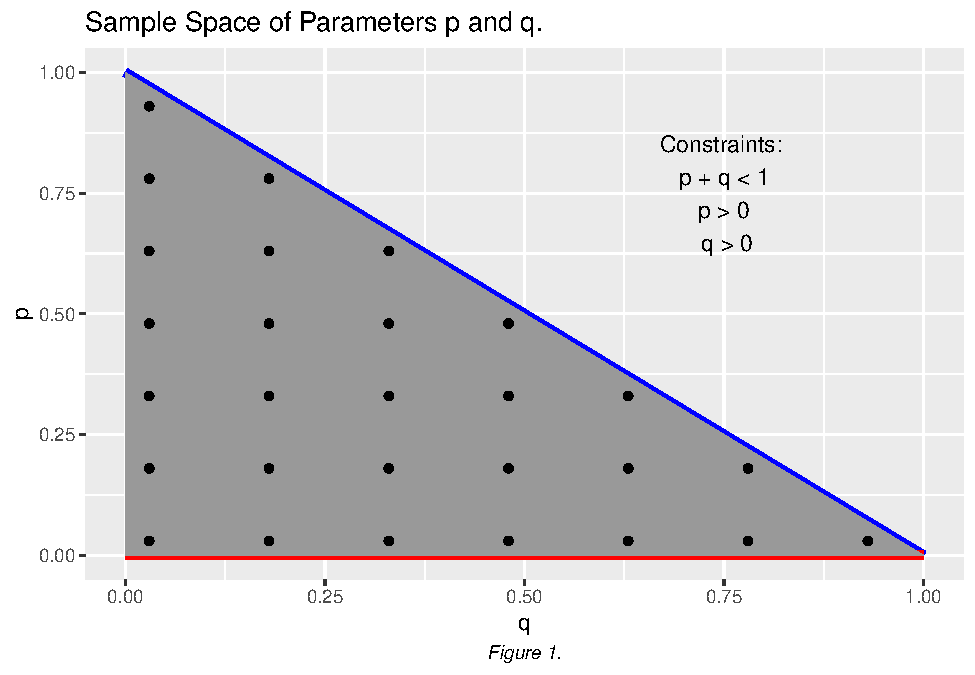
\includegraphics{Genetics_Faizan_HW1_v3_files/figure-latex/unnamed-chunk-1-1.pdf}

\subsection{Selecting Threshold and Accuracy of
Estimates.}\label{selecting-threshold-and-accuracy-of-estimates.}

We select different threshold values for the accuracy of the estimates.
For any practical purpose one would realistically not need an accuracy
of greater than six decimal points \((10^{-5})\). Further, the minimum
accuracy one would need would be at least of two decimal points
\((10^{-2})\). Keeping this range in mind we implement the two
algorithms for threshold values of
\(10^{-3}, 10^{-5}, 10^{-10}, \: and \: \: 10^{-16}\). These values will
allow us to see how the two algorithms' scale as we increase the
accuracy of the estimates.

For each accuracy level we will run both algorithms for all 28 pairs of
initial values. This will give us a combination of \(28 \times 4 = 112\)
runs in total for each algorithm.

\subsection{Data}\label{data}

The data is taken from Bernstein 1925, Sham's book page 44, obtained
from a large random sample of people from Berlin.

\begin{table}[t]

\caption{\label{tab:Data}Table 1: Blood-Type and their counts in the sample population.}
\centering
\begin{tabular}{l|r|r}
\hline
Blood-Type & Count & Frequency\\
\hline
A & 9123 & 0.43\\
\hline
B & 2987 & 0.14\\
\hline
AB & 1269 & 0.06\\
\hline
O & 7725 & 0.37\\
\hline
Total & 21104 & 1.00\\
\hline
\end{tabular}
\end{table}

\section{Results}\label{results}

\subsection{Newton-Raphson Algorithm}\label{newton-raphson-algorithm}

\begin{table}[t]

\caption{\label{tab:unnamed-chunk-4}Table 2: Newton-Raphosn Algorithm: Estimates and number of iterations for different levels of accuracy.}
\centering
\begin{tabular}{c|c|c|c|c|c|c}
\hline
Accuracy & mean p estimate & mean q estimate & mean number of iterations & min iterations & max iterations & n\\
\hline
0.001 & 0.2876857 & 0.1065543 & 6.000000 & 4 & 9 & 27\\
\hline
1e-05 & 0.2876856 & 0.1065550 & 6.925926 & 5 & 10 & 27\\
\hline
1e-10 & 0.2876856 & 0.1065550 & 7.962963 & 6 & 11 & 27\\
\hline
1e-16 & 0.2876856 & 0.1065550 & 8.629630 & 6 & 12 & 27\\
\hline
\end{tabular}
\end{table}

For each accuracy level n should be 28, however, one of the
Newton-Raphson algorithm did not converge for one of the initial points
\((p^{(0)}, q^{(0)}) = (0.18 , 0.33 )\), and the parameters escaped the
sample space, hence, that data point was removed from the results for
each accuracy level so as to not skew the results.

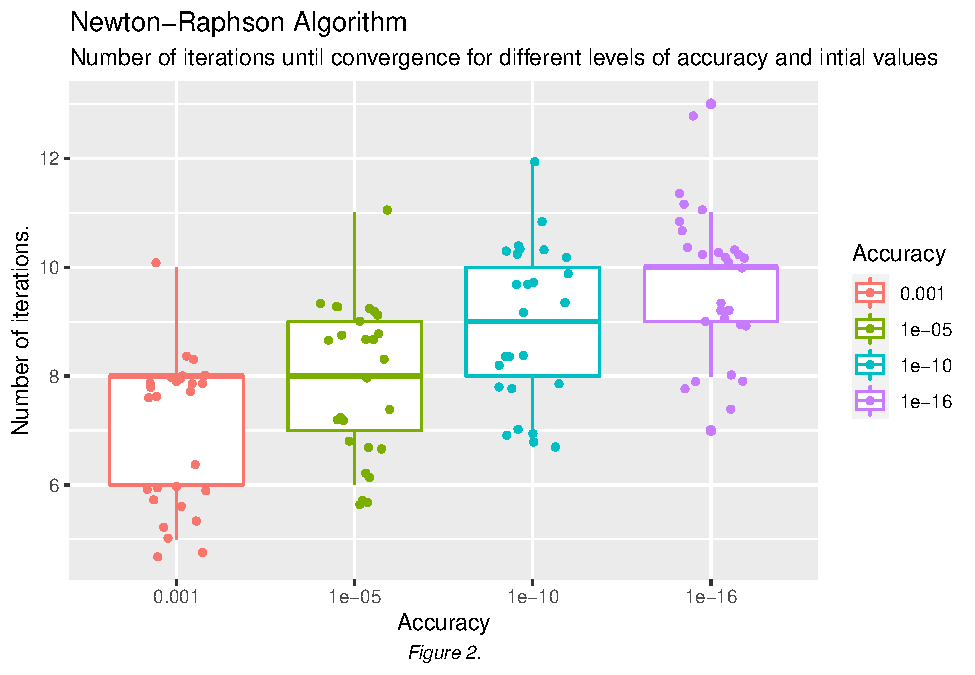
\includegraphics{Genetics_Faizan_HW1_v3_files/figure-latex/unnamed-chunk-5-1.pdf}

Both from Table 2. and Figure 2. above, it can be seen as level of
accuracy for the estimates increase, the average number of iterations
the algorithm takes to converge to the estimates also increases.

\begin{verbatim}
## `geom_smooth()` using formula 'y ~ x'
\end{verbatim}

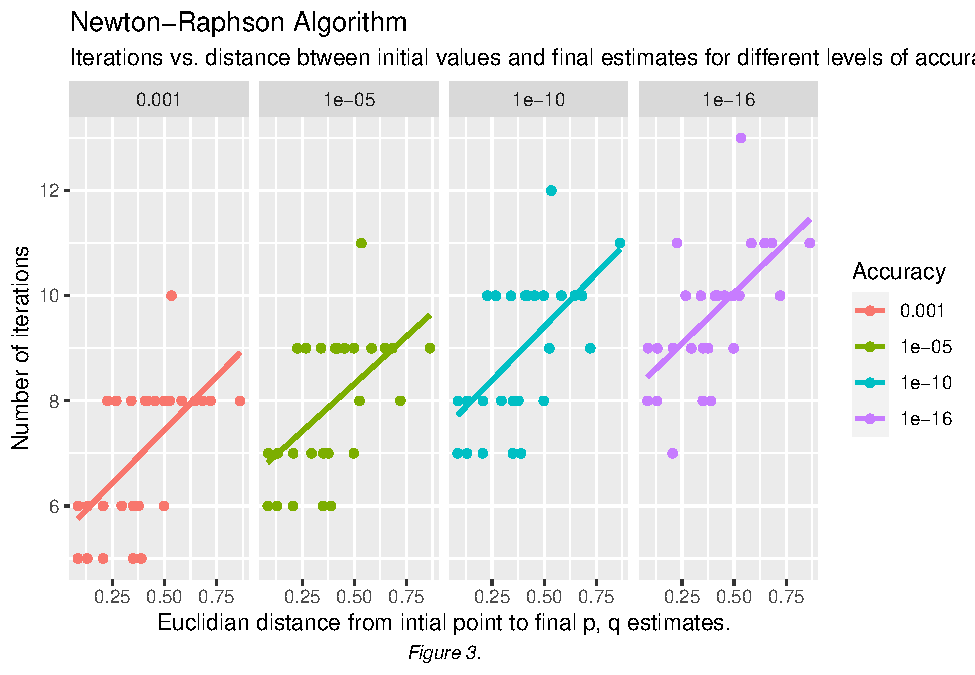
\includegraphics{Genetics_Faizan_HW1_v3_files/figure-latex/unnamed-chunk-6-1.pdf}

We notice from Figure 3, that for any given level of accuracy, the
further the initial values happen to be from the final convergence
estimates of \(\hat{p}\) and \(\hat{q}\), the more iterations on average
the algorithm takes to converge. And from Figure 3, we can also see that
the number of iterations increases linearly with respect to the
euclidean distance between initial value point and final convergence
values of \(\hat{p}\) and \(\hat{q}\).

\subsection{EM Algorithm}\label{em-algorithm}

\begin{table}[t]

\caption{\label{tab:unnamed-chunk-9}Table 3: Expectation-Maximization Algorithm: Estimates and number of iterations for different levels of accuracy.}
\centering
\begin{tabular}{c|c|c|c|c|c|c}
\hline
Accuracy & mean p estimate & mean q estimate & mean number of iterations & min iterations & max iterations & n\\
\hline
0.001 & 0.2877468 & 0.1065609 & 5.714286 & 5 & 8 & 28\\
\hline
1e-05 & 0.2876860 & 0.1065550 & 8.392857 & 6 & 10 & 28\\
\hline
1e-10 & 0.2876856 & 0.1065550 & 15.000000 & 13 & 17 & 28\\
\hline
1e-16 & 0.2876856 & 0.1065550 & 22.964286 & 21 & 25 & 28\\
\hline
\end{tabular}
\end{table}

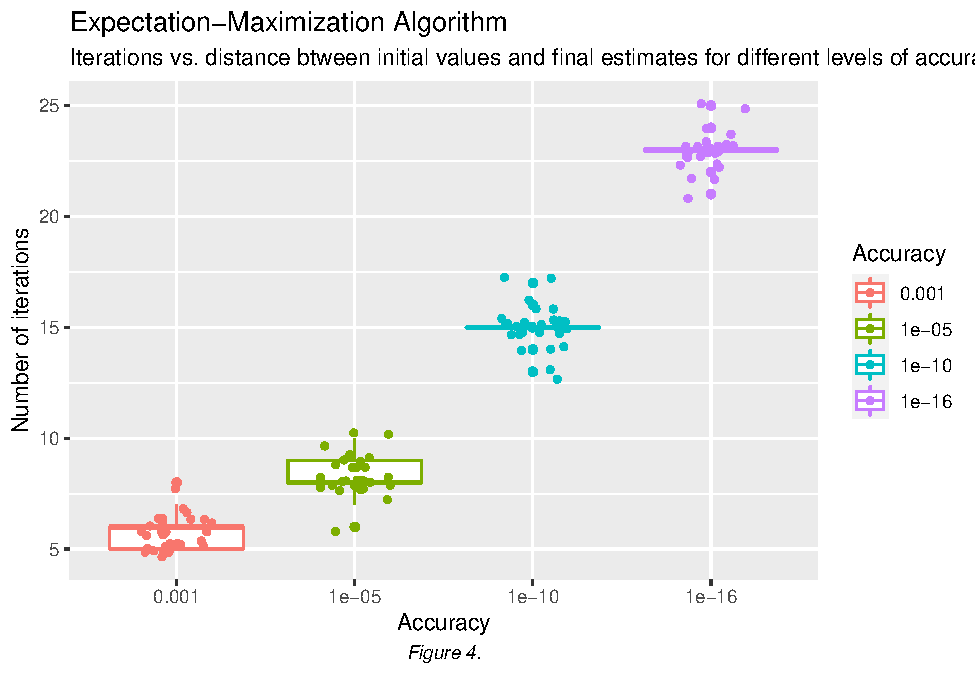
\includegraphics{Genetics_Faizan_HW1_v3_files/figure-latex/unnamed-chunk-10-1.pdf}

We again observe that the higher the accuracy (threshold value) the more
iterations it takes to converge from Table 3 and Figure 4.

\begin{verbatim}
## `geom_smooth()` using formula 'y ~ x'
\end{verbatim}

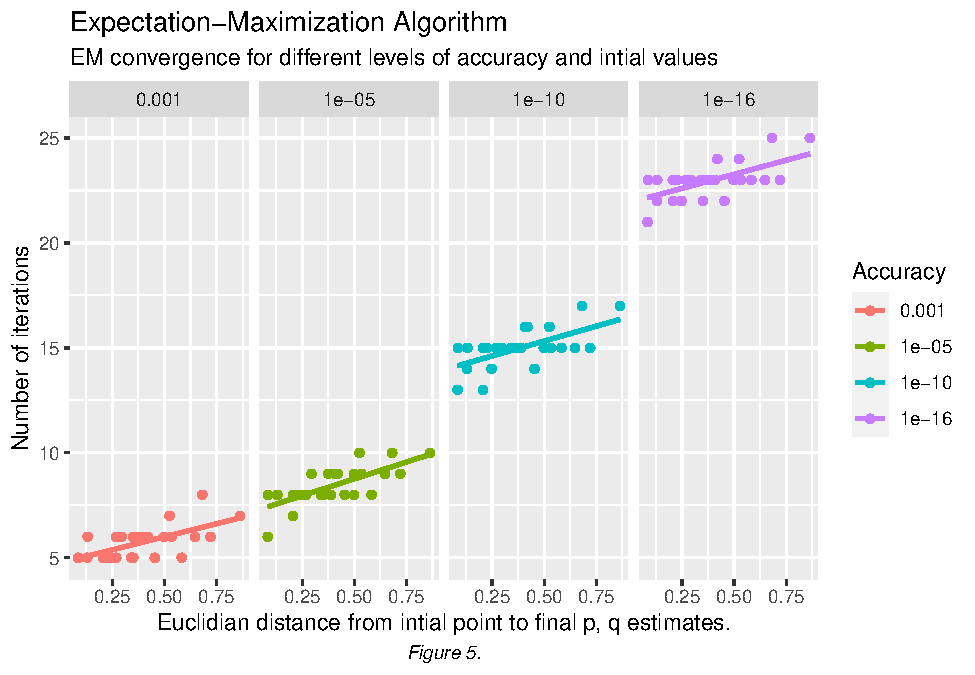
\includegraphics{Genetics_Faizan_HW1_v3_files/figure-latex/unnamed-chunk-11-1.pdf}

For each accuracy level, we notice the further the initial value that we
randomly choose is from the final convergence point the higher the
number of iterations it takes to converge to the estimates: \(\hat{p}\)
and \(\hat{q}\).

Further, we again notice that the higher the accuracy the more
iterations the algorithm takes to converge.

We again notice that for any given level of accuracy, the further the
initial value happen to be from the final convergence estimates of p and
q, the more iterations on average the algorithm takes to converge.

\subsection{Comparing Expectation-Maximization with Newton-Raphson
Algorithm.}\label{comparing-expectation-maximization-with-newton-raphson-algorithm.}

\begin{table}[t]

\caption{\label{tab:unnamed-chunk-12}Table 4: Comparing average iterations, computational time, and estimates of parameters between the EM and NR Algorithms for different levels of accuracy.}
\centering
\begin{tabular}{l|r|r|r|r|r|r|r|r|r|r}
\hline
\multicolumn{1}{c|}{ } & \multicolumn{5}{c|}{Expectation-Maximization Algorithm} & \multicolumn{5}{c}{Newton-Raphson Algorithm} \\
\cline{2-6} \cline{7-11}
\multicolumn{1}{c|}{ } & \multicolumn{5}{c|}{(Computational time: 0.269 sec)} & \multicolumn{5}{c}{(Computational time: 0.443 sec)} \\
\cline{2-6} \cline{7-11}
Accuracy & mean p estimate & mean q estimate & mean iterations & min iterations & max iterations & mean p estimate & mean q estimate & mean iterations & min iterations & max iterations\\
\hline
0.001 & 0.2877468 & 0.1065609 & 5.714286 & 5 & 8 & 0.2876857 & 0.1065543 & 6.000000 & 4 & 9\\
\hline
1e-05 & 0.2876860 & 0.1065550 & 8.392857 & 6 & 10 & 0.2876856 & 0.1065550 & 6.925926 & 5 & 10\\
\hline
1e-10 & 0.2876856 & 0.1065550 & 15.000000 & 13 & 17 & 0.2876856 & 0.1065550 & 7.962963 & 6 & 11\\
\hline
1e-16 & 0.2876856 & 0.1065550 & 22.964286 & 21 & 25 & 0.2876856 & 0.1065550 & 8.629630 & 6 & 12\\
\hline
\end{tabular}
\end{table}

We observe that for high accuracy both algorithms give the same
estimates of \(p\) and \(q\):
\((p^{(final)}, q^{(final)}) = (0.2876856, 0.1065550)\). We also observe
that the EM algorithm has a higher average number of iteration for
convergence for higher accuracy levels compared to the Newton-Raphson
algorithm. This can also be seen in the min and max number of iterations
for different initial values of the two algorithms.

However, we notice that the EM algorithm has smaller computational time
(0.269 sec) compared to Newton-Raphson algorithm (0.443 sec). Although,
this is the run time for code when it is compiled in Rmarkdown through
``knit to HTML''. When we run the two algorithms' codes on the R console
the NR algorithm (0.9153 sec) is faster than the EM algorithm (1.1406
sec).

\section{Discussion}\label{discussion}

\subsection{Comparing Algorithms' parameter estimates, impact of initial
vaules, accuracy levels and computational
time.}\label{comparing-algorithms-parameter-estimates-impact-of-initial-vaules-accuracy-levels-and-computational-time.}

\textbf{Estimates of Parameter Values:} We note that both algorithms
estimate \(\hat{p}\) and \(\hat{q}\) to be equal to 0.2876856 and
0.106555, respectively.

\textbf{Impact of Initial Values:} We also noted that for both
algorithms, and for any given level of accuracy, the further the initial
value happens to be from the final convergence estimates of p and q, the
more iterations on average the algorithms take to converge as can be
seen in Figure 2 and Figure 3. Further, the number of iterations appears
to increase linearly on average with respect to the distance of the
initial values to the final estimates of the parameter values as can be
seen in Figure and Figure .

For the initial pair of \((p^{(0)}, q^{(0)}) = (0.18, 0.43)\) the
Newton-Raphson Algorithm did not converge for any level of accuracy and
the estimates of \(p\) and \(q\) had escaped the parameter space. This
is most likely because at this initial point the Hessian matrix is
singular. For all other initial points the NR algorithm converged. The
EM algorithm, on the other hand converged for all the initial values and
all levels of accuracy.

\textbf{Impact of Accuracy Level:} The higher the accuracy required for
the estimates the more iterations on average it takes for both
algorithms to converge as seen in Figure 2 and Figure 4. This is also
inline with what we would expect.

\textbf{Computational Time:} In terms of computational time the EM
algorithm was faster by -0.2\% compared to NR algorithm when the
RMarkdown file was compiled via ``knit'' and used multi-threading to run
the 112 runs in parallel. However, when we ran both algorithms
sequentially in a for loop in the R console the EM algorithm was 24.5\%
slower compared to the NR algorithm (1.140 sec versus 0.915 sec). We are
not sure what causes this disparity in computational time, but most
likely has to do with running the algorithms in parallel or in sequence.

\textbf{Accuracy Level versus Compuational Time:} In terms of how small
the threshold should be and how much accuracy should be demanded, this
is a trade off between number of iterations and hence computational cost
versus accuracy of estimate acceptable to us. For our small sample size
and only two parameters, both algorithms are relatively fast and we can
require a higher degree of accuracy with both algorithms being very
fast. This trade-off, however, might become important to consider when
we have a high number of parameters to estimate and a large data set.

\subsection{Comments on the stopping
criteria.}\label{comments-on-the-stopping-criteria.}

For the stopping criteria for the implementation of the two algorithms
we took the difference in absolute value between subsequent points. The
distance measured in absolute values is called Manhattan distance.
However, an alternative approach could have been to take the euclidean
distance instead.

Further, looking at two sequential points to determine convergence may
not be the most robust method for determining the stopping criteria,
especially since some algorithms have randomness built in them. Hence, a
stopping criteria that is based on several sequential points of
estimates and calculating two averages and see if the decrease between
the average of two set of sequential points is smaller than a given
threshold or accuracy level would be a more robust stopping criteria
method. This would be more stable as two sequential point estimates can
happen to be randomly very close randomly, but the general trend of the
estimate points decrease is not small enough for a given threshold or
accuracy. Hence, it is a more robust stopping criteria to look at a set
of sequential points and comparing if the average decrease between the
two sets of sequential points is less than a given threshold.

\subsection{Advantages and Disadvantages of the Two
Algorithms}\label{advantages-and-disadvantages-of-the-two-algorithms}

One disadvantage that both algorithms have is that it is impossible to
know if the algorithms, when converged, converged to a local or global
maximum.

One possible way to determine if we have converged to a global maximum
is to do a dense search of the sample space and plot the graph of the
log-likelihood. Through this method one can find the global maximum.

Another disadvantage both algorithms have is that the further the
initial guess (initial point) is from the final estimates of the
parameters the more iterations it will take to converge and more
computational time it will take.

\textbf{NR algorithm:}

An advantage of NR method is that once the iterates are close to the
solution, convergence is very fast\textsuperscript{1}.

The disadvantages of NR algorithm is that if the Hessian matrix does not
exist (indeed possible) or is not invertible then the algorithm will not
work. Also, even if it exists and is invertible, but the number of
parameters is large then the computational load can be very heavy
because of the inverse of the Hessian matrix has to be calculated.

\textbf{EM algorithm:}

The disadvantage of the EM algorithm is that it can be sometime hard to
find the correct statistical expressions for the Expectation and
Maximization steps. However, an advantage is that once the Expectation
and Maximization expressions are found, it is fairly straight forward to
implement.

\section{References}\label{references}

\begin{enumerate}
\def\labelenumi{\arabic{enumi}.}
\tightlist
\item
  Sun, L. (2020, September 16). Lecture Module 3.2: Missing data and EM
  algorithm. University of Toronto, Department of Statistical Sciences,
  FA, Division of Biostatistics, Dalla Lana School of Public Health.
\end{enumerate}

\section{Appendix}\label{appendix}

\subsection{NR Algorithm: Sample Raw
Data.}\label{nr-algorithm-sample-raw-data.}

\begin{verbatim}
##     p0   q0 maxiter epsilon_p epsilon_q ecl_dist_p0q0_to_pq j         p         q Accuracy
## 1 0.03 0.03     100     0.001     0.001               0.269 8 0.2876856 0.1065550    0.001
## 2 0.18 0.03     100     0.001     0.001               0.132 6 0.2876858 0.1065542    0.001
## 3 0.33 0.03     100     0.001     0.001               0.087 6 0.2876859 0.1065540    0.001
## 4 0.48 0.03     100     0.001     0.001               0.207 6 0.2876858 0.1065542    0.001
## 5 0.63 0.03     100     0.001     0.001               0.351 6 0.2876857 0.1065546    0.001
## 6 0.78 0.03     100     0.001     0.001               0.498 6 0.2876856 0.1065550    0.001
\end{verbatim}

\begin{verbatim}
##       p0   q0 maxiter epsilon_p epsilon_q ecl_dist_p0q0_to_pq  j         p        q Accuracy
## 107 0.03 0.63     100     1e-16     1e-16               0.583 11 0.2876856 0.106555    1e-16
## 108 0.18 0.63     100     1e-16     1e-16               0.534 13 0.2876856 0.106555    1e-16
## 109 0.33 0.63     100     1e-16     1e-16               0.525 10 0.2876856 0.106555    1e-16
## 110 0.03 0.78     100     1e-16     1e-16               0.721 10 0.2876856 0.106555    1e-16
## 111 0.18 0.78     100     1e-16     1e-16               0.682 11 0.2876856 0.106555    1e-16
## 112 0.03 0.93     100     1e-16     1e-16               0.863 11 0.2876856 0.106555    1e-16
\end{verbatim}

\subsection{EM Algorithm: Sample Raw
Data.}\label{em-algorithm-sample-raw-data.}

\begin{verbatim}
##     p0   q0 maxiter epsilon_p epsilon_q ecl_dist_p0q0_to_pq j         p         q Accuracy
## 1 0.03 0.03     100     0.001     0.001               0.269 5 0.2874819 0.1065398    0.001
## 2 0.18 0.03     100     0.001     0.001               0.132 6 0.2876447 0.1065515    0.001
## 3 0.33 0.03     100     0.001     0.001               0.088 5 0.2875462 0.1065344    0.001
## 4 0.48 0.03     100     0.001     0.001               0.207 5 0.2876678 0.1065422    0.001
## 5 0.63 0.03     100     0.001     0.001               0.351 5 0.2878273 0.1065528    0.001
## 6 0.78 0.03     100     0.001     0.001               0.498 6 0.2877474 0.1065588    0.001
\end{verbatim}

\begin{verbatim}
##       p0   q0 maxiter epsilon_p epsilon_q ecl_dist_p0q0_to_pq  j         p        q Accuracy
## 107 0.03 0.63     100     1e-16     1e-16               0.583 23 0.2876856 0.106555    1e-16
## 108 0.18 0.63     100     1e-16     1e-16               0.534 23 0.2876856 0.106555    1e-16
## 109 0.33 0.63     100     1e-16     1e-16               0.525 24 0.2876856 0.106555    1e-16
## 110 0.03 0.78     100     1e-16     1e-16               0.721 23 0.2876856 0.106555    1e-16
## 111 0.18 0.78     100     1e-16     1e-16               0.682 25 0.2876856 0.106555    1e-16
## 112 0.03 0.93     100     1e-16     1e-16               0.863 25 0.2876856 0.106555    1e-16
\end{verbatim}


\end{document}
